\documentclass[1p]{elsarticle_modified}
%\bibliographystyle{elsarticle-num}

%\usepackage[colorlinks]{hyperref}
%\usepackage{abbrmath_seonhwa} %\Abb, \Ascr, \Acal ,\Abf, \Afrak
\usepackage{amsfonts}
\usepackage{amssymb}
\usepackage{amsmath}
\usepackage{amsthm}
\usepackage{scalefnt}
\usepackage{amsbsy}
\usepackage{kotex}
\usepackage{caption}
\usepackage{subfig}
\usepackage{color}
\usepackage{graphicx}
\usepackage{xcolor} %% white, black, red, green, blue, cyan, magenta, yellow
\usepackage{float}
\usepackage{setspace}
\usepackage{hyperref}

\usepackage{tikz}
\usetikzlibrary{arrows}

\usepackage{multirow}
\usepackage{array} % fixed length table
\usepackage{hhline}

%%%%%%%%%%%%%%%%%%%%%
\makeatletter
\renewcommand*\env@matrix[1][\arraystretch]{%
	\edef\arraystretch{#1}%
	\hskip -\arraycolsep
	\let\@ifnextchar\new@ifnextchar
	\array{*\c@MaxMatrixCols c}}
\makeatother %https://tex.stackexchange.com/questions/14071/how-can-i-increase-the-line-spacing-in-a-matrix
%%%%%%%%%%%%%%%

\usepackage[normalem]{ulem}

\newcommand{\msout}[1]{\ifmmode\text{\sout{\ensuremath{#1}}}\else\sout{#1}\fi}
%SOURCE: \msout is \stkout macro in https://tex.stackexchange.com/questions/20609/strikeout-in-math-mode

\newcommand{\cancel}[1]{
	\ifmmode
	{\color{red}\msout{#1}}
	\else
	{\color{red}\sout{#1}}
	\fi
}

\newcommand{\add}[1]{
	{\color{blue}\uwave{#1}}
}

\newcommand{\replace}[2]{
	\ifmmode
	{\color{red}\msout{#1}}{\color{blue}\uwave{#2}}
	\else
	{\color{red}\sout{#1}}{\color{blue}\uwave{#2}}
	\fi
}

\newcommand{\Sol}{\mathcal{S}} %segment
\newcommand{\D}{D} %diagram
\newcommand{\A}{\mathcal{A}} %arc


%%%%%%%%%%%%%%%%%%%%%%%%%%%%%5 test

\def\sl{\operatorname{\textup{SL}}(2,\Cbb)}
\def\psl{\operatorname{\textup{PSL}}(2,\Cbb)}
\def\quan{\mkern 1mu \triangleright \mkern 1mu}

\theoremstyle{definition}
\newtheorem{thm}{Theorem}[section]
\newtheorem{prop}[thm]{Proposition}
\newtheorem{lem}[thm]{Lemma}
\newtheorem{ques}[thm]{Question}
\newtheorem{cor}[thm]{Corollary}
\newtheorem{defn}[thm]{Definition}
\newtheorem{exam}[thm]{Example}
\newtheorem{rmk}[thm]{Remark}
\newtheorem{alg}[thm]{Algorithm}

\newcommand{\I}{\sqrt{-1}}
\begin{document}

%\begin{frontmatter}
%
%\title{Boundary parabolic representations of knots up to 8 crossings}
%
%%% Group authors per affiliation:
%\author{Yunhi Cho} 
%\address{Department of Mathematics, University of Seoul, Seoul, Korea}
%\ead{yhcho@uos.ac.kr}
%
%
%\author{Seonhwa Kim} %\fnref{s_kim}}
%\address{Center for Geometry and Physics, Institute for Basic Science, Pohang, 37673, Korea}
%\ead{ryeona17@ibs.re.kr}
%
%\author{Hyuk Kim}
%\address{Department of Mathematical Sciences, Seoul National University, Seoul 08826, Korea}
%\ead{hyukkim@snu.ac.kr}
%
%\author{Seokbeom Yoon}
%\address{Department of Mathematical Sciences, Seoul National University, Seoul, 08826,  Korea}
%\ead{sbyoon15@snu.ac.kr}
%
%\begin{abstract}
%We find all boundary parabolic representation of knots up to 8 crossings.
%
%\end{abstract}
%\begin{keyword}
%    \MSC[2010] 57M25 
%\end{keyword}
%
%\end{frontmatter}

%\linenumbers
%\tableofcontents
%
\newcommand\colored[1]{\textcolor{white}{\rule[-0.35ex]{0.8em}{1.4ex}}\kern-0.8em\color{red} #1}%
%\newcommand\colored[1]{\textcolor{white}{ #1}\kern-2.17ex	\textcolor{white}{ #1}\kern-1.81ex	\textcolor{white}{ #1}\kern-2.15ex\color{red}#1	}

{\Large $\underline{11n_{103}~(K11n_{103})}$}

\setlength{\tabcolsep}{10pt}
\renewcommand{\arraystretch}{1.6}
\vspace{1cm}\begin{tabular}{m{100pt}>{\centering\arraybackslash}m{274pt}}
\multirow{5}{120pt}{
	\centering
	\includegraphics[width=112pt]{../../../GIT/diagram.site/Diagrams/png/719_11n_103.png}\\
\ \ \ A knot diagram\footnotemark}&
\allowdisplaybreaks
\textbf{Linearized knot diagam} \\
\cline{2-2}
 &
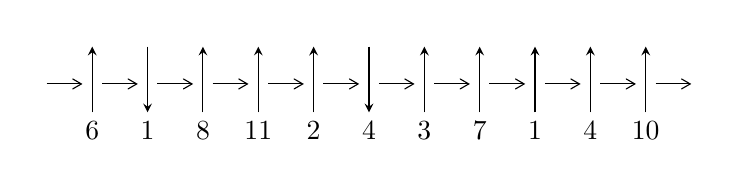
\begin{tikzpicture}[x=20pt, y=17pt]
	% nodes
	\node (C0) at (0, 0) {};
	\node (C1) at (1, 0) {};
	\node (C1U) at (1, +1) {};
	\node (C1D) at (1, -1) {6};

	\node (C2) at (2, 0) {};
	\node (C2U) at (2, +1) {};
	\node (C2D) at (2, -1) {1};

	\node (C3) at (3, 0) {};
	\node (C3U) at (3, +1) {};
	\node (C3D) at (3, -1) {8};

	\node (C4) at (4, 0) {};
	\node (C4U) at (4, +1) {};
	\node (C4D) at (4, -1) {11};

	\node (C5) at (5, 0) {};
	\node (C5U) at (5, +1) {};
	\node (C5D) at (5, -1) {2};

	\node (C6) at (6, 0) {};
	\node (C6U) at (6, +1) {};
	\node (C6D) at (6, -1) {4};

	\node (C7) at (7, 0) {};
	\node (C7U) at (7, +1) {};
	\node (C7D) at (7, -1) {3};

	\node (C8) at (8, 0) {};
	\node (C8U) at (8, +1) {};
	\node (C8D) at (8, -1) {7};

	\node (C9) at (9, 0) {};
	\node (C9U) at (9, +1) {};
	\node (C9D) at (9, -1) {1};

	\node (C10) at (10, 0) {};
	\node (C10U) at (10, +1) {};
	\node (C10D) at (10, -1) {4};

	\node (C11) at (11, 0) {};
	\node (C11U) at (11, +1) {};
	\node (C11D) at (11, -1) {10};
	\node (C12) at (12, 0) {};

	% arrows
	\draw[->,>={angle 60}]
	(C0) edge (C1) (C1) edge (C2) (C2) edge (C3) (C3) edge (C4) (C4) edge (C5) (C5) edge (C6) (C6) edge (C7) (C7) edge (C8) (C8) edge (C9) (C9) edge (C10) (C10) edge (C11) (C11) edge (C12) ;	\draw[->,>=stealth]
	(C1D) edge (C1U) (C2U) edge (C2D) (C3D) edge (C3U) (C4D) edge (C4U) (C5D) edge (C5U) (C6U) edge (C6D) (C7D) edge (C7U) (C8D) edge (C8U) (C9D) edge (C9U) (C10D) edge (C10U) (C11D) edge (C11U) ;
	\end{tikzpicture} \\
\hhline{~~} \\& 
\textbf{Solving Sequence} \\ \cline{2-2} 
 &
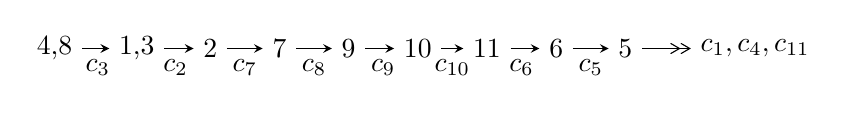
\begin{tikzpicture}[x=25pt, y=7pt]
	% node
	\node (A0) at (-1/8, 0) {4,8};
	\node (A1) at (17/16, 0) {1,3};
	\node (A2) at (17/8, 0) {2};
	\node (A3) at (25/8, 0) {7};
	\node (A4) at (33/8, 0) {9};
	\node (A5) at (41/8, 0) {10};
	\node (A6) at (49/8, 0) {11};
	\node (A7) at (57/8, 0) {6};
	\node (A8) at (65/8, 0) {5};
	\node (C1) at (1/2, -1) {$c_{3}$};
	\node (C2) at (13/8, -1) {$c_{2}$};
	\node (C3) at (21/8, -1) {$c_{7}$};
	\node (C4) at (29/8, -1) {$c_{8}$};
	\node (C5) at (37/8, -1) {$c_{9}$};
	\node (C6) at (45/8, -1) {$c_{10}$};
	\node (C7) at (53/8, -1) {$c_{6}$};
	\node (C8) at (61/8, -1) {$c_{5}$};
	\node (A9) at (10, 0) {$c_{1},c_{4},c_{11}$};

	% edge
	\draw[->,>=stealth]	
	(A0) edge (A1) (A1) edge (A2) (A2) edge (A3) (A3) edge (A4) (A4) edge (A5) (A5) edge (A6) (A6) edge (A7) (A7) edge (A8) ;
	\draw[->>,>={angle 60}]	
	(A8) edge (A9);
\end{tikzpicture} \\ 

\end{tabular} \\

\footnotetext{
The image of knot diagram is generated by the software ``\textbf{Draw programme}" developed by Andrew Bartholomew(\url{http://www.layer8.co.uk/maths/draw/index.htm\#Running-draw}), where we modified some parts for our purpose(\url{https://github.com/CATsTAILs/LinksPainter}).
}\phantom \\ \newline 
\centering \textbf{Ideals for irreducible components\footnotemark of $X_{\text{par}}$} 
 
\begin{align*}
I^u_{1}&=\langle 
- u^3+b+u,\;- u^{11}+3 u^9+u^8-3 u^7-2 u^6-2 u^5+u^4+2 u^3+2 u^2+2 a+2 u-1,\\
\phantom{I^u_{1}}&\phantom{= \langle  }u^{12}-4 u^{10}+7 u^8- u^7-4 u^6+3 u^5-2 u^4-3 u^3+3 u^2-1\rangle \\
I^u_{2}&=\langle 
1323539668 u^{27}+477420100 u^{26}+\cdots+373862627 b+2208818501,\\
\phantom{I^u_{2}}&\phantom{= \langle  }3623527383 u^{27}+808013199 u^{26}+\cdots+373862627 a+4728861229,\;u^{28}+u^{27}+\cdots- u^2+1\rangle \\
I^u_{3}&=\langle 
- u^3+b+u,\;- u^3+u^2+a-1,\;u^4- u^2+1\rangle \\
I^u_{4}&=\langle 
b- u,\;u^3+u^2+a- u-1,\;u^4- u^2+1\rangle \\
\\
\end{align*}
\raggedright * 4 irreducible components of $\dim_{\mathbb{C}}=0$, with total 48 representations.\\
\footnotetext{All coefficients of polynomials are rational numbers. But the coefficients are sometimes approximated in decimal forms when there is not enough margin.}
\newpage
\renewcommand{\arraystretch}{1}
\centering \section*{I. $I^u_{1}= \langle - u^3+b+u,\;- u^{11}+3 u^9+\cdots+2 a-1,\;u^{12}-4 u^{10}+\cdots+3 u^2-1 \rangle$}
\flushleft \textbf{(i) Arc colorings}\\
\begin{tabular}{m{7pt} m{180pt} m{7pt} m{180pt} }
\flushright $a_{4}=$&$\begin{pmatrix}1\\0\end{pmatrix}$ \\
\flushright $a_{8}=$&$\begin{pmatrix}0\\u\end{pmatrix}$ \\
\flushright $a_{1}=$&$\begin{pmatrix}\frac{1}{2} u^{11}-\frac{3}{2} u^9+\cdots- u+\frac{1}{2}\\u^3- u\end{pmatrix}$ \\
\flushright $a_{3}=$&$\begin{pmatrix}1\\u^2\end{pmatrix}$ \\
\flushright $a_{2}=$&$\begin{pmatrix}u^{11}-\frac{1}{2} u^{10}+\cdots-\frac{1}{2} u+\frac{1}{2}\\-\frac{1}{2} u^{10}+\frac{1}{2} u^9+\cdots-\frac{1}{2} u-\frac{1}{2}\end{pmatrix}$ \\
\flushright $a_{7}=$&$\begin{pmatrix}- u\\- u^3+u\end{pmatrix}$ \\
\flushright $a_{9}=$&$\begin{pmatrix}u^3\\u^5- u^3+u\end{pmatrix}$ \\
\flushright $a_{10}=$&$\begin{pmatrix}-\frac{1}{2} u^{11}+\frac{1}{2} u^{10}+\cdots-\frac{1}{2} u^2-\frac{1}{2} u\\u\end{pmatrix}$ \\
\flushright $a_{11}=$&$\begin{pmatrix}-\frac{1}{2} u^{11}+\frac{1}{2} u^{10}+\cdots-\frac{1}{2} u^2+\frac{1}{2} u\\u\end{pmatrix}$ \\
\flushright $a_{6}=$&$\begin{pmatrix}- u^3\\- u^3+u\end{pmatrix}$ \\
\flushright $a_{5}=$&$\begin{pmatrix}-\frac{1}{2} u^{11}+\frac{3}{2} u^9+\cdots-2 u^2+\frac{3}{2}\\- u^2\end{pmatrix}$\\ \flushright $a_{5}=$&$\begin{pmatrix}-\frac{1}{2} u^{11}+\frac{3}{2} u^9+\cdots-2 u^2+\frac{3}{2}\\- u^2\end{pmatrix}$\\&\end{tabular}
\flushleft \textbf{(ii) Obstruction class $= -1$}\\~\\
\flushleft \textbf{(iii) Cusp Shapes $= u^{11}+2 u^{10}- u^9-7 u^8-3 u^7+10 u^6+8 u^5-5 u^4+2 u^3-8 u+9$}\\~\\
\newpage\renewcommand{\arraystretch}{1}
\flushleft \textbf{(iv) u-Polynomials at the component}\newline \\
\begin{tabular}{m{50pt}|m{274pt}}
Crossings & \hspace{64pt}u-Polynomials at each crossing \\
\hline $$\begin{aligned}c_{1},c_{5}\end{aligned}$$&$\begin{aligned}
&u^{12}-5 u^{11}+\cdots+20 u-4
\end{aligned}$\\
\hline $$\begin{aligned}c_{2}\end{aligned}$$&$\begin{aligned}
&u^{12}+5 u^{11}+\cdots-88 u+16
\end{aligned}$\\
\hline $$\begin{aligned}c_{3},c_{4},c_{7}\\c_{10}\end{aligned}$$&$\begin{aligned}
&u^{12}-4 u^{10}+7 u^8+u^7-4 u^6-3 u^5-2 u^4+3 u^3+3 u^2-1
\end{aligned}$\\
\hline $$\begin{aligned}c_{6}\end{aligned}$$&$\begin{aligned}
&u^{12}+8 u^{10}+\cdots-2 u+1
\end{aligned}$\\
\hline $$\begin{aligned}c_{8},c_{9},c_{11}\end{aligned}$$&$\begin{aligned}
&u^{12}-8 u^{11}+\cdots-6 u+1
\end{aligned}$\\
\hline
\end{tabular}\\~\\
\newpage\renewcommand{\arraystretch}{1}
\flushleft \textbf{(v) Riley Polynomials at the component}\newline \\
\begin{tabular}{m{50pt}|m{274pt}}
Crossings & \hspace{64pt}Riley Polynomials at each crossing \\
\hline $$\begin{aligned}c_{1},c_{5}\end{aligned}$$&$\begin{aligned}
&y^{12}+5 y^{11}+\cdots-88 y+16
\end{aligned}$\\
\hline $$\begin{aligned}c_{2}\end{aligned}$$&$\begin{aligned}
&y^{12}+5 y^{11}+\cdots-13088 y+256
\end{aligned}$\\
\hline $$\begin{aligned}c_{3},c_{4},c_{7}\\c_{10}\end{aligned}$$&$\begin{aligned}
&y^{12}-8 y^{11}+\cdots-6 y+1
\end{aligned}$\\
\hline $$\begin{aligned}c_{6}\end{aligned}$$&$\begin{aligned}
&y^{12}+16 y^{11}+\cdots-10 y+1
\end{aligned}$\\
\hline $$\begin{aligned}c_{8},c_{9},c_{11}\end{aligned}$$&$\begin{aligned}
&y^{12}-4 y^{11}+\cdots-10 y+1
\end{aligned}$\\
\hline
\end{tabular}\\~\\
\newpage\flushleft \textbf{(vi) Complex Volumes and Cusp Shapes}
$$\begin{array}{c|c|c}  
\text{Solutions to }I^u_{1}& \I (\text{vol} + \sqrt{-1}CS) & \text{Cusp shape}\\
 \hline 
\begin{aligned}
u &= -1.070850 + 0.293331 I \\
a &= \phantom{-}0.88474 + 1.47446 I \\
b &= \phantom{-}0.119301 + 0.690537 I\end{aligned}
 & \phantom{-}0.88385 - 3.90933 I & \phantom{-}11.22062 + 4.69963 I \\ \hline\begin{aligned}
u &= -1.070850 - 0.293331 I \\
a &= \phantom{-}0.88474 - 1.47446 I \\
b &= \phantom{-}0.119301 - 0.690537 I\end{aligned}
 & \phantom{-}0.88385 + 3.90933 I & \phantom{-}11.22062 - 4.69963 I \\ \hline\begin{aligned}
u &= \phantom{-}0.123324 + 0.852412 I \\
a &= \phantom{-}0.190031 + 0.083600 I \\
b &= -0.39027 - 1.43289 I\end{aligned}
 & \phantom{-}1.59916 - 2.93187 I & \phantom{-}4.52833 + 2.34392 I \\ \hline\begin{aligned}
u &= \phantom{-}0.123324 - 0.852412 I \\
a &= \phantom{-}0.190031 - 0.083600 I \\
b &= -0.39027 + 1.43289 I\end{aligned}
 & \phantom{-}1.59916 + 2.93187 I & \phantom{-}4.52833 - 2.34392 I \\ \hline\begin{aligned}
u &= \phantom{-}1.18703\phantom{ +0.000000I} \\
a &= -0.319027\phantom{ +0.000000I} \\
b &= \phantom{-}0.485533\phantom{ +0.000000I}\end{aligned}
 & \phantom{-}5.86925\phantom{ +0.000000I} & \phantom{-}15.2180\phantom{ +0.000000I} \\ \hline\begin{aligned}
u &= \phantom{-}0.583435 + 0.389720 I \\
a &= -0.490222 - 1.302820 I \\
b &= -0.650675 - 0.050933 I\end{aligned}
 & -2.15137 + 2.12179 I & \phantom{-}2.80850 - 2.85099 I \\ \hline\begin{aligned}
u &= \phantom{-}0.583435 - 0.389720 I \\
a &= -0.490222 + 1.302820 I \\
b &= -0.650675 + 0.050933 I\end{aligned}
 & -2.15137 - 2.12179 I & \phantom{-}2.80850 + 2.85099 I \\ \hline\begin{aligned}
u &= -1.237240 + 0.570642 I \\
a &= -1.14325 + 1.84850 I \\
b &= \phantom{-}0.55197 + 1.86409 I\end{aligned}
 & \phantom{-}8.0502 - 13.4162 I & \phantom{-}9.70040 + 8.08040 I \\ \hline\begin{aligned}
u &= -1.237240 - 0.570642 I \\
a &= -1.14325 - 1.84850 I \\
b &= \phantom{-}0.55197 - 1.86409 I\end{aligned}
 & \phantom{-}8.0502 + 13.4162 I & \phantom{-}9.70040 - 8.08040 I \\ \hline\begin{aligned}
u &= \phantom{-}1.278420 + 0.477758 I \\
a &= \phantom{-}0.80625 + 1.61595 I \\
b &= -0.06443 + 1.75567 I\end{aligned}
 & \phantom{-}9.66215 + 6.36480 I & \phantom{-}11.90320 - 3.80747 I\\
 \hline 
 \end{array}$$\newpage$$\begin{array}{c|c|c}  
\text{Solutions to }I^u_{1}& \I (\text{vol} + \sqrt{-1}CS) & \text{Cusp shape}\\
 \hline 
\begin{aligned}
u &= \phantom{-}1.278420 - 0.477758 I \\
a &= \phantom{-}0.80625 - 1.61595 I \\
b &= -0.06443 - 1.75567 I\end{aligned}
 & \phantom{-}9.66215 - 6.36480 I & \phantom{-}11.90320 + 3.80747 I \\ \hline\begin{aligned}
u &= -0.541203\phantom{ +0.000000I} \\
a &= \phantom{-}0.823936\phantom{ +0.000000I} \\
b &= \phantom{-}0.382684\phantom{ +0.000000I}\end{aligned}
 & \phantom{-}0.811000\phantom{ +0.000000I} & \phantom{-}12.4600\phantom{ +0.000000I}\\
 \hline 
 \end{array}$$\newpage\newpage\renewcommand{\arraystretch}{1}
\centering \section*{II. $I^u_{2}= \langle 1.32\times10^{9} u^{27}+4.77\times10^{8} u^{26}+\cdots+3.74\times10^{8} b+2.21\times10^{9},\;3.62\times10^{9} u^{27}+8.08\times10^{8} u^{26}+\cdots+3.74\times10^{8} a+4.73\times10^{9},\;u^{28}+u^{27}+\cdots- u^2+1 \rangle$}
\flushleft \textbf{(i) Arc colorings}\\
\begin{tabular}{m{7pt} m{180pt} m{7pt} m{180pt} }
\flushright $a_{4}=$&$\begin{pmatrix}1\\0\end{pmatrix}$ \\
\flushright $a_{8}=$&$\begin{pmatrix}0\\u\end{pmatrix}$ \\
\flushright $a_{1}=$&$\begin{pmatrix}-9.69214 u^{27}-2.16126 u^{26}+\cdots+21.1172 u-12.6487\\-3.54018 u^{27}-1.27699 u^{26}+\cdots+6.39747 u-5.90810\end{pmatrix}$ \\
\flushright $a_{3}=$&$\begin{pmatrix}1\\u^2\end{pmatrix}$ \\
\flushright $a_{2}=$&$\begin{pmatrix}-11.1683 u^{27}-2.69831 u^{26}+\cdots+24.1271 u-14.6661\\-2.00633 u^{27}-0.821463 u^{26}+\cdots+3.57032 u-3.52639\end{pmatrix}$ \\
\flushright $a_{7}=$&$\begin{pmatrix}- u\\- u^3+u\end{pmatrix}$ \\
\flushright $a_{9}=$&$\begin{pmatrix}u^3\\u^5- u^3+u\end{pmatrix}$ \\
\flushright $a_{10}=$&$\begin{pmatrix}8.82770 u^{27}+2.98162 u^{26}+\cdots-18.8225 u+11.0259\\-1.96759 u^{27}-0.358100 u^{26}+\cdots+2.54082 u-1.68118\end{pmatrix}$ \\
\flushright $a_{11}=$&$\begin{pmatrix}6.86011 u^{27}+2.62352 u^{26}+\cdots-16.2817 u+9.34470\\-1.96759 u^{27}-0.358100 u^{26}+\cdots+2.54082 u-1.68118\end{pmatrix}$ \\
\flushright $a_{6}=$&$\begin{pmatrix}- u^3\\- u^3+u\end{pmatrix}$ \\
\flushright $a_{5}=$&$\begin{pmatrix}0.604072 u^{27}-0.672673 u^{26}+\cdots+2.58371 u+1.13808\\4.82738 u^{27}+1.39404 u^{26}+\cdots-6.80258 u+5.67111\end{pmatrix}$\\ \flushright $a_{5}=$&$\begin{pmatrix}0.604072 u^{27}-0.672673 u^{26}+\cdots+2.58371 u+1.13808\\4.82738 u^{27}+1.39404 u^{26}+\cdots-6.80258 u+5.67111\end{pmatrix}$\\&\end{tabular}
\flushleft \textbf{(ii) Obstruction class $= -1$}\\~\\
\flushleft \textbf{(iii) Cusp Shapes $= \frac{3205496750}{373862627} u^{27}+\frac{1277226600}{373862627} u^{26}+\cdots-\frac{4858013364}{373862627} u+\frac{5377018252}{373862627}$}\\~\\
\newpage\renewcommand{\arraystretch}{1}
\flushleft \textbf{(iv) u-Polynomials at the component}\newline \\
\begin{tabular}{m{50pt}|m{274pt}}
Crossings & \hspace{64pt}u-Polynomials at each crossing \\
\hline $$\begin{aligned}c_{1},c_{5}\end{aligned}$$&$\begin{aligned}
&(u^{14}+2 u^{13}+\cdots+2 u^2+1)^{2}
\end{aligned}$\\
\hline $$\begin{aligned}c_{2}\end{aligned}$$&$\begin{aligned}
&(u^{14}+4 u^{13}+\cdots+4 u+1)^{2}
\end{aligned}$\\
\hline $$\begin{aligned}c_{3},c_{4},c_{7}\\c_{10}\end{aligned}$$&$\begin{aligned}
&u^{28}- u^{27}+\cdots- u^2+1
\end{aligned}$\\
\hline $$\begin{aligned}c_{6}\end{aligned}$$&$\begin{aligned}
&u^{28}-3 u^{27}+\cdots-64 u+17
\end{aligned}$\\
\hline $$\begin{aligned}c_{8},c_{9},c_{11}\end{aligned}$$&$\begin{aligned}
&u^{28}-15 u^{27}+\cdots-2 u+1
\end{aligned}$\\
\hline
\end{tabular}\\~\\
\newpage\renewcommand{\arraystretch}{1}
\flushleft \textbf{(v) Riley Polynomials at the component}\newline \\
\begin{tabular}{m{50pt}|m{274pt}}
Crossings & \hspace{64pt}Riley Polynomials at each crossing \\
\hline $$\begin{aligned}c_{1},c_{5}\end{aligned}$$&$\begin{aligned}
&(y^{14}+4 y^{13}+\cdots+4 y+1)^{2}
\end{aligned}$\\
\hline $$\begin{aligned}c_{2}\end{aligned}$$&$\begin{aligned}
&(y^{14}+16 y^{13}+\cdots+28 y+1)^{2}
\end{aligned}$\\
\hline $$\begin{aligned}c_{3},c_{4},c_{7}\\c_{10}\end{aligned}$$&$\begin{aligned}
&y^{28}-15 y^{27}+\cdots-2 y+1
\end{aligned}$\\
\hline $$\begin{aligned}c_{6}\end{aligned}$$&$\begin{aligned}
&y^{28}+21 y^{27}+\cdots-3178 y+289
\end{aligned}$\\
\hline $$\begin{aligned}c_{8},c_{9},c_{11}\end{aligned}$$&$\begin{aligned}
&y^{28}-3 y^{27}+\cdots+78 y+1
\end{aligned}$\\
\hline
\end{tabular}\\~\\
\newpage\flushleft \textbf{(vi) Complex Volumes and Cusp Shapes}
$$\begin{array}{c|c|c}  
\text{Solutions to }I^u_{2}& \I (\text{vol} + \sqrt{-1}CS) & \text{Cusp shape}\\
 \hline 
\begin{aligned}
u &= -0.946438 + 0.337794 I \\
a &= \phantom{-}0.900026 + 0.777028 I \\
b &= \phantom{-}1.205620 - 0.251783 I\end{aligned}
 & \phantom{-}0.225291 - 0.283453 I & \phantom{-}9.98682 + 1.62016 I \\ \hline\begin{aligned}
u &= -0.946438 - 0.337794 I \\
a &= \phantom{-}0.900026 - 0.777028 I \\
b &= \phantom{-}1.205620 + 0.251783 I\end{aligned}
 & \phantom{-}0.225291 + 0.283453 I & \phantom{-}9.98682 - 1.62016 I \\ \hline\begin{aligned}
u &= -0.772691 + 0.621111 I \\
a &= \phantom{-}0.901192 + 0.236459 I \\
b &= \phantom{-}0.422650 - 0.531395 I\end{aligned}
 & \phantom{-}0.225291 + 0.283453 I & \phantom{-}9.98682 - 1.62016 I \\ \hline\begin{aligned}
u &= -0.772691 - 0.621111 I \\
a &= \phantom{-}0.901192 - 0.236459 I \\
b &= \phantom{-}0.422650 + 0.531395 I\end{aligned}
 & \phantom{-}0.225291 - 0.283453 I & \phantom{-}9.98682 + 1.62016 I \\ \hline\begin{aligned}
u &= \phantom{-}0.772763 + 0.566548 I \\
a &= \phantom{-}0.120522 - 0.536761 I \\
b &= -0.246731 + 0.289946 I\end{aligned}
 & -1.79770 + 2.20081 I & \phantom{-}2.89649 - 4.56299 I \\ \hline\begin{aligned}
u &= \phantom{-}0.772763 - 0.566548 I \\
a &= \phantom{-}0.120522 + 0.536761 I \\
b &= -0.246731 - 0.289946 I\end{aligned}
 & -1.79770 - 2.20081 I & \phantom{-}2.89649 + 4.56299 I \\ \hline\begin{aligned}
u &= -0.195025 + 0.938101 I \\
a &= \phantom{-}0.0007473 + 0.1043940 I \\
b &= -0.39042 + 1.67653 I\end{aligned}
 & \phantom{-}4.87993 + 7.94699 I & \phantom{-}7.43585 - 5.15066 I \\ \hline\begin{aligned}
u &= -0.195025 - 0.938101 I \\
a &= \phantom{-}0.0007473 - 0.1043940 I \\
b &= -0.39042 - 1.67653 I\end{aligned}
 & \phantom{-}4.87993 - 7.94699 I & \phantom{-}7.43585 + 5.15066 I \\ \hline\begin{aligned}
u &= \phantom{-}0.006608 + 0.931399 I \\
a &= \phantom{-}0.426144 + 0.112166 I \\
b &= -0.082738 + 1.405960 I\end{aligned}
 & \phantom{-}5.74815 - 1.35811 I & \phantom{-}8.91559 + 0.70318 I \\ \hline\begin{aligned}
u &= \phantom{-}0.006608 - 0.931399 I \\
a &= \phantom{-}0.426144 - 0.112166 I \\
b &= -0.082738 - 1.405960 I\end{aligned}
 & \phantom{-}5.74815 + 1.35811 I & \phantom{-}8.91559 - 0.70318 I\\
 \hline 
 \end{array}$$\newpage$$\begin{array}{c|c|c}  
\text{Solutions to }I^u_{2}& \I (\text{vol} + \sqrt{-1}CS) & \text{Cusp shape}\\
 \hline 
\begin{aligned}
u &= -0.852569 + 0.695292 I \\
a &= \phantom{-}0.089649 - 0.218079 I \\
b &= -0.324576 - 0.830884 I\end{aligned}
 & \phantom{-}0.44424 - 5.41715 I & \phantom{-}9.45457 + 7.85187 I \\ \hline\begin{aligned}
u &= -0.852569 - 0.695292 I \\
a &= \phantom{-}0.089649 + 0.218079 I \\
b &= -0.324576 + 0.830884 I\end{aligned}
 & \phantom{-}0.44424 + 5.41715 I & \phantom{-}9.45457 - 7.85187 I \\ \hline\begin{aligned}
u &= \phantom{-}0.961456 + 0.569453 I \\
a &= \phantom{-}0.875348 - 0.814669 I \\
b &= \phantom{-}0.344071 - 0.029085 I\end{aligned}
 & -1.13610 + 2.11470 I & \phantom{-}7.32861 - 1.96391 I \\ \hline\begin{aligned}
u &= \phantom{-}0.961456 - 0.569453 I \\
a &= \phantom{-}0.875348 + 0.814669 I \\
b &= \phantom{-}0.344071 + 0.029085 I\end{aligned}
 & -1.13610 - 2.11470 I & \phantom{-}7.32861 + 1.96391 I \\ \hline\begin{aligned}
u &= \phantom{-}1.056900 + 0.376008 I \\
a &= \phantom{-}0.37905 - 1.49389 I \\
b &= \phantom{-}1.46933 - 0.48475 I\end{aligned}
 & \phantom{-}0.44424 + 5.41715 I & \phantom{-}9.45457 - 7.85187 I \\ \hline\begin{aligned}
u &= \phantom{-}1.056900 - 0.376008 I \\
a &= \phantom{-}0.37905 + 1.49389 I \\
b &= \phantom{-}1.46933 + 0.48475 I\end{aligned}
 & \phantom{-}0.44424 - 5.41715 I & \phantom{-}9.45457 + 7.85187 I \\ \hline\begin{aligned}
u &= -0.733151 + 0.047660 I \\
a &= \phantom{-}0.43746 - 2.41615 I \\
b &= -1.008020 - 0.825090 I\end{aligned}
 & -1.13610 - 2.11470 I & \phantom{-}7.32861 + 1.96391 I \\ \hline\begin{aligned}
u &= -0.733151 - 0.047660 I \\
a &= \phantom{-}0.43746 + 2.41615 I \\
b &= -1.008020 + 0.825090 I\end{aligned}
 & -1.13610 + 2.11470 I & \phantom{-}7.32861 - 1.96391 I \\ \hline\begin{aligned}
u &= -1.245820 + 0.402354 I \\
a &= \phantom{-}0.95707 - 1.63848 I \\
b &= -0.02380 - 1.73927 I\end{aligned}
 & \phantom{-}5.74815 - 1.35811 I & \phantom{-}8.91559 + 0.70318 I \\ \hline\begin{aligned}
u &= -1.245820 - 0.402354 I \\
a &= \phantom{-}0.95707 + 1.63848 I \\
b &= -0.02380 + 1.73927 I\end{aligned}
 & \phantom{-}5.74815 + 1.35811 I & \phantom{-}8.91559 - 0.70318 I\\
 \hline 
 \end{array}$$\newpage$$\begin{array}{c|c|c}  
\text{Solutions to }I^u_{2}& \I (\text{vol} + \sqrt{-1}CS) & \text{Cusp shape}\\
 \hline 
\begin{aligned}
u &= \phantom{-}1.223100 + 0.521275 I \\
a &= -0.95325 - 1.80175 I \\
b &= \phantom{-}0.70249 - 1.65662 I\end{aligned}
 & \phantom{-}4.87993 + 7.94699 I & \phantom{-}7.43585 - 5.15066 I \\ \hline\begin{aligned}
u &= \phantom{-}1.223100 - 0.521275 I \\
a &= -0.95325 + 1.80175 I \\
b &= \phantom{-}0.70249 + 1.65662 I\end{aligned}
 & \phantom{-}4.87993 - 7.94699 I & \phantom{-}7.43585 + 5.15066 I \\ \hline\begin{aligned}
u &= \phantom{-}1.307490 + 0.340934 I \\
a &= \phantom{-}0.96986 + 1.76670 I \\
b &= \phantom{-}0.01577 + 1.74521 I\end{aligned}
 & \phantom{-}9.73046 - 3.61450 I & \phantom{-}11.98207 + 2.36533 I \\ \hline\begin{aligned}
u &= \phantom{-}1.307490 - 0.340934 I \\
a &= \phantom{-}0.96986 - 1.76670 I \\
b &= \phantom{-}0.01577 - 1.74521 I\end{aligned}
 & \phantom{-}9.73046 + 3.61450 I & \phantom{-}11.98207 - 2.36533 I \\ \hline\begin{aligned}
u &= -1.283470 + 0.468890 I \\
a &= -0.96559 + 1.49926 I \\
b &= \phantom{-}0.47177 + 1.36795 I\end{aligned}
 & \phantom{-}9.73046 - 3.61450 I & \phantom{-}11.98207 + 2.36533 I \\ \hline\begin{aligned}
u &= -1.283470 - 0.468890 I \\
a &= -0.96559 - 1.49926 I \\
b &= \phantom{-}0.47177 - 1.36795 I\end{aligned}
 & \phantom{-}9.73046 + 3.61450 I & \phantom{-}11.98207 - 2.36533 I \\ \hline\begin{aligned}
u &= \phantom{-}0.200841 + 0.299347 I \\
a &= \phantom{-}1.36178 + 1.98186 I \\
b &= -1.055410 - 0.266567 I\end{aligned}
 & -1.79770 - 2.20081 I & \phantom{-}2.89649 + 4.56299 I \\ \hline\begin{aligned}
u &= \phantom{-}0.200841 - 0.299347 I \\
a &= \phantom{-}1.36178 - 1.98186 I \\
b &= -1.055410 + 0.266567 I\end{aligned}
 & -1.79770 + 2.20081 I & \phantom{-}2.89649 - 4.56299 I\\
 \hline 
 \end{array}$$\newpage\newpage\renewcommand{\arraystretch}{1}
\centering \section*{III. $I^u_{3}= \langle - u^3+b+u,\;- u^3+u^2+a-1,\;u^4- u^2+1 \rangle$}
\flushleft \textbf{(i) Arc colorings}\\
\begin{tabular}{m{7pt} m{180pt} m{7pt} m{180pt} }
\flushright $a_{4}=$&$\begin{pmatrix}1\\0\end{pmatrix}$ \\
\flushright $a_{8}=$&$\begin{pmatrix}0\\u\end{pmatrix}$ \\
\flushright $a_{1}=$&$\begin{pmatrix}u^3- u^2+1\\u^3- u\end{pmatrix}$ \\
\flushright $a_{3}=$&$\begin{pmatrix}1\\u^2\end{pmatrix}$ \\
\flushright $a_{2}=$&$\begin{pmatrix}u^3- u^2+2\\u^3+u^2- u\end{pmatrix}$ \\
\flushright $a_{7}=$&$\begin{pmatrix}- u\\- u^3+u\end{pmatrix}$ \\
\flushright $a_{9}=$&$\begin{pmatrix}u^3\\0\end{pmatrix}$ \\
\flushright $a_{10}=$&$\begin{pmatrix}2 u^3- u+1\\- u\end{pmatrix}$ \\
\flushright $a_{11}=$&$\begin{pmatrix}2 u^3-2 u+1\\- u\end{pmatrix}$ \\
\flushright $a_{6}=$&$\begin{pmatrix}- u^3\\- u^3+u\end{pmatrix}$ \\
\flushright $a_{5}=$&$\begin{pmatrix}u-1\\- u^2\end{pmatrix}$\\ \flushright $a_{5}=$&$\begin{pmatrix}u-1\\- u^2\end{pmatrix}$\\&\end{tabular}
\flushleft \textbf{(ii) Obstruction class $= 1$}\\~\\
\flushleft \textbf{(iii) Cusp Shapes $= -8 u^2+8$}\\~\\
\newpage\renewcommand{\arraystretch}{1}
\flushleft \textbf{(iv) u-Polynomials at the component}\newline \\
\begin{tabular}{m{50pt}|m{274pt}}
Crossings & \hspace{64pt}u-Polynomials at each crossing \\
\hline $$\begin{aligned}c_{1},c_{5}\end{aligned}$$&$\begin{aligned}
&(u^2+1)^2
\end{aligned}$\\
\hline $$\begin{aligned}c_{2}\end{aligned}$$&$\begin{aligned}
&(u+1)^4
\end{aligned}$\\
\hline $$\begin{aligned}c_{3},c_{4},c_{6}\\c_{7},c_{10}\end{aligned}$$&$\begin{aligned}
&u^4- u^2+1
\end{aligned}$\\
\hline $$\begin{aligned}c_{8},c_{11}\end{aligned}$$&$\begin{aligned}
&(u^2- u+1)^2
\end{aligned}$\\
\hline $$\begin{aligned}c_{9}\end{aligned}$$&$\begin{aligned}
&(u^2+u+1)^2
\end{aligned}$\\
\hline
\end{tabular}\\~\\
\newpage\renewcommand{\arraystretch}{1}
\flushleft \textbf{(v) Riley Polynomials at the component}\newline \\
\begin{tabular}{m{50pt}|m{274pt}}
Crossings & \hspace{64pt}Riley Polynomials at each crossing \\
\hline $$\begin{aligned}c_{1},c_{5}\end{aligned}$$&$\begin{aligned}
&(y+1)^4
\end{aligned}$\\
\hline $$\begin{aligned}c_{2}\end{aligned}$$&$\begin{aligned}
&(y-1)^4
\end{aligned}$\\
\hline $$\begin{aligned}c_{3},c_{4},c_{6}\\c_{7},c_{10}\end{aligned}$$&$\begin{aligned}
&(y^2- y+1)^2
\end{aligned}$\\
\hline $$\begin{aligned}c_{8},c_{9},c_{11}\end{aligned}$$&$\begin{aligned}
&(y^2+y+1)^2
\end{aligned}$\\
\hline
\end{tabular}\\~\\
\newpage\flushleft \textbf{(vi) Complex Volumes and Cusp Shapes}
$$\begin{array}{c|c|c}  
\text{Solutions to }I^u_{3}& \I (\text{vol} + \sqrt{-1}CS) & \text{Cusp shape}\\
 \hline 
\begin{aligned}
u &= \phantom{-}0.866025 + 0.500000 I \\
a &= \phantom{-}0.500000 + 0.133975 I \\
b &= -0.866025 + 0.500000 I\end{aligned}
 & -1.64493 + 4.05977 I & \phantom{-}4.00000 - 6.92820 I \\ \hline\begin{aligned}
u &= \phantom{-}0.866025 - 0.500000 I \\
a &= \phantom{-}0.500000 - 0.133975 I \\
b &= -0.866025 - 0.500000 I\end{aligned}
 & -1.64493 - 4.05977 I & \phantom{-}4.00000 + 6.92820 I \\ \hline\begin{aligned}
u &= -0.866025 + 0.500000 I \\
a &= \phantom{-}0.50000 + 1.86603 I \\
b &= \phantom{-}0.866025 + 0.500000 I\end{aligned}
 & -1.64493 - 4.05977 I & \phantom{-}4.00000 + 6.92820 I \\ \hline\begin{aligned}
u &= -0.866025 - 0.500000 I \\
a &= \phantom{-}0.50000 - 1.86603 I \\
b &= \phantom{-}0.866025 - 0.500000 I\end{aligned}
 & -1.64493 + 4.05977 I & \phantom{-}4.00000 - 6.92820 I\\
 \hline 
 \end{array}$$\newpage\newpage\renewcommand{\arraystretch}{1}
\centering \section*{IV. $I^u_{4}= \langle b- u,\;u^3+u^2+a- u-1,\;u^4- u^2+1 \rangle$}
\flushleft \textbf{(i) Arc colorings}\\
\begin{tabular}{m{7pt} m{180pt} m{7pt} m{180pt} }
\flushright $a_{4}=$&$\begin{pmatrix}1\\0\end{pmatrix}$ \\
\flushright $a_{8}=$&$\begin{pmatrix}0\\u\end{pmatrix}$ \\
\flushright $a_{1}=$&$\begin{pmatrix}- u^3- u^2+u+1\\u\end{pmatrix}$ \\
\flushright $a_{3}=$&$\begin{pmatrix}1\\u^2\end{pmatrix}$ \\
\flushright $a_{2}=$&$\begin{pmatrix}- u^3- u^2+u+2\\u^2+u\end{pmatrix}$ \\
\flushright $a_{7}=$&$\begin{pmatrix}- u\\- u^3+u\end{pmatrix}$ \\
\flushright $a_{9}=$&$\begin{pmatrix}u^3\\0\end{pmatrix}$ \\
\flushright $a_{10}=$&$\begin{pmatrix}- u^2\\- u^3+u\end{pmatrix}$ \\
\flushright $a_{11}=$&$\begin{pmatrix}- u^3- u^2+u\\- u^3+u\end{pmatrix}$ \\
\flushright $a_{6}=$&$\begin{pmatrix}- u^3\\- u^3+u\end{pmatrix}$ \\
\flushright $a_{5}=$&$\begin{pmatrix}u^2+u\\u^2-1\end{pmatrix}$\\ \flushright $a_{5}=$&$\begin{pmatrix}u^2+u\\u^2-1\end{pmatrix}$\\&\end{tabular}
\flushleft \textbf{(ii) Obstruction class $= 1$}\\~\\
\flushleft \textbf{(iii) Cusp Shapes $= 4$}\\~\\
\newpage\renewcommand{\arraystretch}{1}
\flushleft \textbf{(iv) u-Polynomials at the component}\newline \\
\begin{tabular}{m{50pt}|m{274pt}}
Crossings & \hspace{64pt}u-Polynomials at each crossing \\
\hline $$\begin{aligned}c_{1},c_{5}\end{aligned}$$&$\begin{aligned}
&(u^2+1)^2
\end{aligned}$\\
\hline $$\begin{aligned}c_{2}\end{aligned}$$&$\begin{aligned}
&(u+1)^4
\end{aligned}$\\
\hline $$\begin{aligned}c_{3},c_{4},c_{6}\\c_{7},c_{10}\end{aligned}$$&$\begin{aligned}
&u^4- u^2+1
\end{aligned}$\\
\hline $$\begin{aligned}c_{8},c_{11}\end{aligned}$$&$\begin{aligned}
&(u^2- u+1)^2
\end{aligned}$\\
\hline $$\begin{aligned}c_{9}\end{aligned}$$&$\begin{aligned}
&(u^2+u+1)^2
\end{aligned}$\\
\hline
\end{tabular}\\~\\
\newpage\renewcommand{\arraystretch}{1}
\flushleft \textbf{(v) Riley Polynomials at the component}\newline \\
\begin{tabular}{m{50pt}|m{274pt}}
Crossings & \hspace{64pt}Riley Polynomials at each crossing \\
\hline $$\begin{aligned}c_{1},c_{5}\end{aligned}$$&$\begin{aligned}
&(y+1)^4
\end{aligned}$\\
\hline $$\begin{aligned}c_{2}\end{aligned}$$&$\begin{aligned}
&(y-1)^4
\end{aligned}$\\
\hline $$\begin{aligned}c_{3},c_{4},c_{6}\\c_{7},c_{10}\end{aligned}$$&$\begin{aligned}
&(y^2- y+1)^2
\end{aligned}$\\
\hline $$\begin{aligned}c_{8},c_{9},c_{11}\end{aligned}$$&$\begin{aligned}
&(y^2+y+1)^2
\end{aligned}$\\
\hline
\end{tabular}\\~\\
\newpage\flushleft \textbf{(vi) Complex Volumes and Cusp Shapes}
$$\begin{array}{c|c|c}  
\text{Solutions to }I^u_{4}& \I (\text{vol} + \sqrt{-1}CS) & \text{Cusp shape}\\
 \hline 
\begin{aligned}
u &= \phantom{-}0.866025 + 0.500000 I \\
a &= \phantom{-}1.36603 - 1.36603 I \\
b &= \phantom{-}0.866025 + 0.500000 I\end{aligned}
 & -1.64493\phantom{ +0.000000I} & \phantom{-}4.00000\phantom{ +0.000000I} \\ \hline\begin{aligned}
u &= \phantom{-}0.866025 - 0.500000 I \\
a &= \phantom{-}1.36603 + 1.36603 I \\
b &= \phantom{-}0.866025 - 0.500000 I\end{aligned}
 & -1.64493\phantom{ +0.000000I} & \phantom{-}4.00000\phantom{ +0.000000I} \\ \hline\begin{aligned}
u &= -0.866025 + 0.500000 I \\
a &= -0.366025 + 0.366025 I \\
b &= -0.866025 + 0.500000 I\end{aligned}
 & -1.64493\phantom{ +0.000000I} & \phantom{-}4.00000\phantom{ +0.000000I} \\ \hline\begin{aligned}
u &= -0.866025 - 0.500000 I \\
a &= -0.366025 - 0.366025 I \\
b &= -0.866025 - 0.500000 I\end{aligned}
 & -1.64493\phantom{ +0.000000I} & \phantom{-}4.00000\phantom{ +0.000000I}\\
 \hline 
 \end{array}$$\newpage
\newpage\renewcommand{\arraystretch}{1}
\centering \section*{ V. u-Polynomials}
\begin{tabular}{m{50pt}|m{274pt}}
Crossings & \hspace{64pt}u-Polynomials at each crossing \\
\hline $$\begin{aligned}c_{1},c_{5}\end{aligned}$$&$\begin{aligned}
&((u^2+1)^4)(u^{12}-5 u^{11}+\cdots+20 u-4)(u^{14}+2 u^{13}+\cdots+2 u^2+1)^{2}
\end{aligned}$\\
\hline $$\begin{aligned}c_{2}\end{aligned}$$&$\begin{aligned}
&((u+1)^8)(u^{12}+5 u^{11}+\cdots-88 u+16)(u^{14}+4 u^{13}+\cdots+4 u+1)^{2}
\end{aligned}$\\
\hline $$\begin{aligned}c_{3},c_{4},c_{7}\\c_{10}\end{aligned}$$&$\begin{aligned}
&((u^4- u^2+1)^2)(u^{12}-4 u^{10}+\cdots+3 u^2-1)\\
&\cdot(u^{28}- u^{27}+\cdots- u^2+1)
\end{aligned}$\\
\hline $$\begin{aligned}c_{6}\end{aligned}$$&$\begin{aligned}
&((u^4- u^2+1)^2)(u^{12}+8 u^{10}+\cdots-2 u+1)(u^{28}-3 u^{27}+\cdots-64 u+17)
\end{aligned}$\\
\hline $$\begin{aligned}c_{8},c_{11}\end{aligned}$$&$\begin{aligned}
&((u^2- u+1)^4)(u^{12}-8 u^{11}+\cdots-6 u+1)(u^{28}-15 u^{27}+\cdots-2 u+1)
\end{aligned}$\\
\hline $$\begin{aligned}c_{9}\end{aligned}$$&$\begin{aligned}
&((u^2+u+1)^4)(u^{12}-8 u^{11}+\cdots-6 u+1)(u^{28}-15 u^{27}+\cdots-2 u+1)
\end{aligned}$\\
\hline
\end{tabular}\newpage\renewcommand{\arraystretch}{1}
\centering \section*{ VI. Riley Polynomials}
\begin{tabular}{m{50pt}|m{274pt}}
Crossings & \hspace{64pt}Riley Polynomials at each crossing \\
\hline $$\begin{aligned}c_{1},c_{5}\end{aligned}$$&$\begin{aligned}
&((y+1)^8)(y^{12}+5 y^{11}+\cdots-88 y+16)(y^{14}+4 y^{13}+\cdots+4 y+1)^{2}
\end{aligned}$\\
\hline $$\begin{aligned}c_{2}\end{aligned}$$&$\begin{aligned}
&((y-1)^8)(y^{12}+5 y^{11}+\cdots-13088 y+256)\\
&\cdot(y^{14}+16 y^{13}+\cdots+28 y+1)^{2}
\end{aligned}$\\
\hline $$\begin{aligned}c_{3},c_{4},c_{7}\\c_{10}\end{aligned}$$&$\begin{aligned}
&((y^2- y+1)^4)(y^{12}-8 y^{11}+\cdots-6 y+1)(y^{28}-15 y^{27}+\cdots-2 y+1)
\end{aligned}$\\
\hline $$\begin{aligned}c_{6}\end{aligned}$$&$\begin{aligned}
&((y^2- y+1)^4)(y^{12}+16 y^{11}+\cdots-10 y+1)\\
&\cdot(y^{28}+21 y^{27}+\cdots-3178 y+289)
\end{aligned}$\\
\hline $$\begin{aligned}c_{8},c_{9},c_{11}\end{aligned}$$&$\begin{aligned}
&((y^2+y+1)^4)(y^{12}-4 y^{11}+\cdots-10 y+1)(y^{28}-3 y^{27}+\cdots+78 y+1)
\end{aligned}$\\
\hline
\end{tabular}
\vskip 2pc
\end{document}